\documentclass[12pt]{article}
\usepackage{tikz}
\usepackage{amsmath}
% Underlining package
\usepackage{ulem}
\usetikzlibrary{calc}
\usepackage[a4paper, portrait, margin=1cm]{geometry}
\usepackage{fancyhdr}

\def \HeadingAnswers {\section*{\Large Name: \underline{\hspace{8cm}} \hfill Date: \underline{\hspace{3cm}}} \vspace{-3mm}
{Angles in a Triangle: Answers} \vspace{1pt}\hrule}

% raise footer with page number; no header
\fancypagestyle{myfancypagestyle}{
  \fancyhf{}% clear all header and footer fields
  \renewcommand{\headrulewidth}{0pt} % no rule under header
  \fancyfoot[C] {\thepage} \setlength{\footskip}{14.5pt} % raise page number 6pt
}
\pagestyle{myfancypagestyle}  % apply myfancypagestyle

\newcounter{minipagecount}

\begin{document}
\HeadingAnswers
\vspace{8mm}

\begin{minipage}{0.55\textwidth}
  \refstepcounter{minipagecount}
  \noindent{(\theminipagecount)}\quad
  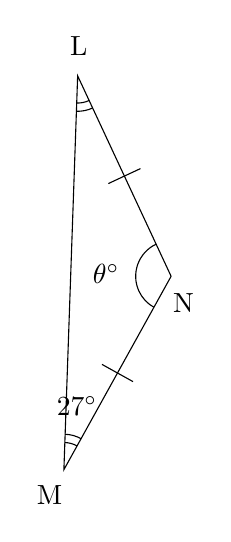
\begin{tikzpicture}[scale=1.5, baseline=(current bounding box.north)]

    \begin{scope}[rotate=268]
      \coordinate (A) at (0,0);
      \coordinate (B) at (3.3358087076495626,0);
      \coordinate (C) at (intersection cs: first line={(A)--($(A)+(27:4cm)$)}, second line={(B)--($(B)+(180-27:4cm)$)});
      \draw (A) -- (B) -- (C) -- cycle;

      % Mark angles with arcs; double arc for equal angles
      \draw ($(A)!0.23cm!(B)$) arc [start angle=0, end angle=27, radius=0.23cm];
      \draw ($(A)!0.3cm!(B)$) arc [start angle=0, end angle=27, radius=0.3cm];
      \draw ($(B)!0.23cm!(C)$) arc [start angle=180-27, end angle=180, radius=0.23cm];
      \draw ($(B)!0.3cm!(C)$) arc [start angle=180-27, end angle=180, radius=0.3cm];
      \draw ($(C)!0.3cm!(A)$) arc [start angle=180+27, end angle=360-27, radius=0.3cm];

      % Label angles
      \node at ($(A)!-0.25cm!(B)$) {L};
      \node at ($(B)!-0.25cm!(C)$) {M};
      \node at ($(C)!-0.25cm!(A)$) {N};

      % Mark angles in degrees
      \coordinate (midBC) at ($(B)!0.5!(C)$);
      \node at ($(A)!0.55cm!(midBC)$) {};

      \coordinate (midAC) at ($(A)!0.5!(C)$);
      \node at ($(B)!0.55cm!(midAC)$) {$27^\circ$};

      \coordinate (midAB) at ($(A)!0.5!(B)$);
      \node at ($(C)!0.55cm!(midAB)$) {$\theta^\circ$};

      % Draw hash mark perpendicular to line AB at its midpoint
      \draw[black] ($(midAC)!1.5mm!90:(A)$)--($(midAC)!1.5mm!-90:(A)$);

      % Add hash marks on side AC
      \draw[black] ($(midBC)!1.5mm!90:(B)$)--($(midBC)!1.5mm!-90:(B)$);

    \end{scope}
  \end{tikzpicture}
\end{minipage}%
\hfill
\begin{minipage}{0.4\textwidth}
  \begin{align*}
    \text{$\theta^\circ$} &= 180^\circ - (\angle \text{L} + \angle \text{M}) \\
    &= 180^\circ - (27^\circ + 27^\circ) \\
    &= 180^\circ - 54^\circ \\
    &= 126^\circ
  \end{align*}
\end{minipage}

\begin{minipage}{0.55\textwidth}
  \refstepcounter{minipagecount}
  \noindent{(\theminipagecount)}\quad
  \begin{tikzpicture}[scale=1.5, baseline=(current bounding box.north)]

    \begin{scope}[rotate=317]
      \coordinate (A) at (0,0);
      \coordinate (B) at (3.014764869491839,0);
      \coordinate (C) at (intersection cs: first line={(A)--($(A)+(53:4cm)$)}, second line={(B)--($(B)+(180-53:4cm)$)});
      \draw (A) -- (B) -- (C) -- cycle;

      % Mark angles with arcs; double arc for equal angles
      \draw ($(A)!0.23cm!(B)$) arc [start angle=0, end angle=53, radius=0.23cm];
      \draw ($(A)!0.3cm!(B)$) arc [start angle=0, end angle=53, radius=0.3cm];
      \draw ($(B)!0.23cm!(C)$) arc [start angle=180-53, end angle=180, radius=0.23cm];
      \draw ($(B)!0.3cm!(C)$) arc [start angle=180-53, end angle=180, radius=0.3cm];
      \draw ($(C)!0.3cm!(A)$) arc [start angle=180+53, end angle=360-53, radius=0.3cm];

      % Label angles
      \node at ($(A)!-0.25cm!(B)$) {A};
      \node at ($(B)!-0.25cm!(C)$) {B};
      \node at ($(C)!-0.25cm!(A)$) {C};

      % Mark angles in degrees
      \coordinate (midBC) at ($(B)!0.5!(C)$);
      \node at ($(A)!0.55cm!(midBC)$) {$\theta^\circ$};

      \coordinate (midAC) at ($(A)!0.5!(C)$);
      \node at ($(B)!0.55cm!(midAC)$) {};

      \coordinate (midAB) at ($(A)!0.5!(B)$);
      \node at ($(C)!0.55cm!(midAB)$) {$74^\circ$};

      % Draw hash mark perpendicular to line AB at its midpoint
      \draw[black] ($(midAC)!1.5mm!90:(A)$)--($(midAC)!1.5mm!-90:(A)$);

      % Add hash marks on side AC
      \draw[black] ($(midBC)!1.5mm!90:(B)$)--($(midBC)!1.5mm!-90:(B)$);

    \end{scope}
  \end{tikzpicture}
\end{minipage}%
\hfill
\begin{minipage}{0.4\textwidth}
  \begin{align*}
    \text{$\theta^\circ$} &= \frac{(180^\circ - \angle \text{C})}{2} \\
    &= \frac{(180^\circ - 74^\circ)}{2} \\
    &= \frac{106^\circ}{2} \\
    &= 53^\circ
  \end{align*}
\end{minipage}

\begin{minipage}{0.55\textwidth}
  \refstepcounter{minipagecount}
  \noindent{(\theminipagecount)}\quad
  \begin{tikzpicture}[scale=1.5, baseline=(current bounding box.north)]

    \begin{scope}[rotate=314]
      \coordinate (A) at (0,0);
      \coordinate (B) at (3.698829928261037,0);
      \coordinate (C) at (intersection cs: first line={(A)--($(A)+(58:4cm)$)}, second line={(B)--($(B)+(180-58:4cm)$)});
      \draw (A) -- (B) -- (C) -- cycle;

      % Mark angles with arcs; double arc for equal angles
      \draw ($(A)!0.23cm!(B)$) arc [start angle=0, end angle=58, radius=0.23cm];
      \draw ($(A)!0.3cm!(B)$) arc [start angle=0, end angle=58, radius=0.3cm];
      \draw ($(B)!0.23cm!(C)$) arc [start angle=180-58, end angle=180, radius=0.23cm];
      \draw ($(B)!0.3cm!(C)$) arc [start angle=180-58, end angle=180, radius=0.3cm];
      \draw ($(C)!0.3cm!(A)$) arc [start angle=180+58, end angle=360-58, radius=0.3cm];

      % Label angles
      \node at ($(A)!-0.25cm!(B)$) {G};
      \node at ($(B)!-0.25cm!(C)$) {F};
      \node at ($(C)!-0.25cm!(A)$) {H};

      % Mark angles in degrees
      \coordinate (midBC) at ($(B)!0.5!(C)$);
      \node at ($(A)!0.55cm!(midBC)$) {$\theta^\circ$};

      \coordinate (midAC) at ($(A)!0.5!(C)$);
      \node at ($(B)!0.55cm!(midAC)$) {};

      \coordinate (midAB) at ($(A)!0.5!(B)$);
      \node at ($(C)!0.55cm!(midAB)$) {$64^\circ$};

      % Draw hash mark perpendicular to line AB at its midpoint
      \draw[black] ($(midAC)!1.5mm!90:(A)$)--($(midAC)!1.5mm!-90:(A)$);

      % Add hash marks on side AC
      \draw[black] ($(midBC)!1.5mm!90:(B)$)--($(midBC)!1.5mm!-90:(B)$);

    \end{scope}
  \end{tikzpicture}
\end{minipage}%
\hfill
\begin{minipage}{0.4\textwidth}
  \begin{align*}
    \text{$\theta^\circ$} &= \frac{(180^\circ - \angle \text{H})}{2} \\
    &= \frac{(180^\circ - 64^\circ)}{2} \\
    &= \frac{116^\circ}{2} \\
    &= 58^\circ
  \end{align*}
\end{minipage}

\begin{minipage}{0.55\textwidth}
  \refstepcounter{minipagecount}
  \noindent{(\theminipagecount)}\quad
  \begin{tikzpicture}[scale=1.5, baseline=(current bounding box.north)]

    \begin{scope}[rotate=202]
      \coordinate (A) at (0,0);
      \coordinate (B) at (3.282422598576085,0);
      \coordinate (C) at (intersection cs: first line={(A)--($(A)+(61:4cm)$)}, second line={(B)--($(B)+(180-61:4cm)$)});
      \draw (A) -- (B) -- (C) -- cycle;

      % Mark angles with arcs; double arc for equal angles
      \draw ($(A)!0.23cm!(B)$) arc [start angle=0, end angle=61, radius=0.23cm];
      \draw ($(A)!0.3cm!(B)$) arc [start angle=0, end angle=61, radius=0.3cm];
      \draw ($(B)!0.23cm!(C)$) arc [start angle=180-61, end angle=180, radius=0.23cm];
      \draw ($(B)!0.3cm!(C)$) arc [start angle=180-61, end angle=180, radius=0.3cm];
      \draw ($(C)!0.3cm!(A)$) arc [start angle=180+61, end angle=360-61, radius=0.3cm];

      % Label angles
      \node at ($(A)!-0.25cm!(B)$) {R};
      \node at ($(B)!-0.25cm!(C)$) {T};
      \node at ($(C)!-0.25cm!(A)$) {S};

      % Mark angles in degrees
      \coordinate (midBC) at ($(B)!0.5!(C)$);
      \node at ($(A)!0.55cm!(midBC)$) {};

      \coordinate (midAC) at ($(A)!0.5!(C)$);
      \node at ($(B)!0.55cm!(midAC)$) {$\theta^\circ$};

      \coordinate (midAB) at ($(A)!0.5!(B)$);
      \node at ($(C)!0.55cm!(midAB)$) {$58^\circ$};

      % Draw hash mark perpendicular to line AB at its midpoint
      \draw[black] ($(midAC)!1.5mm!90:(A)$)--($(midAC)!1.5mm!-90:(A)$);

      % Add hash marks on side AC
      \draw[black] ($(midBC)!1.5mm!90:(B)$)--($(midBC)!1.5mm!-90:(B)$);

    \end{scope}
  \end{tikzpicture}
\end{minipage}%
\hfill
\begin{minipage}{0.4\textwidth}
  \begin{align*}
    \text{$\theta^\circ$} &= \frac{(180^\circ - \angle \text{S})}{2} \\
    &= \frac{(180^\circ - 58^\circ)}{2} \\
    &= \frac{122^\circ}{2} \\
    &= 61^\circ
  \end{align*}
\end{minipage}

\begin{minipage}{0.55\textwidth}
  \refstepcounter{minipagecount}
  \noindent{(\theminipagecount)}\quad
  \begin{tikzpicture}[scale=1.5, baseline=(current bounding box.north)]

    \begin{scope}[rotate=217]
      \coordinate (A) at (0,0);
      \coordinate (B) at (3.5421165755066077,0);
      \coordinate (C) at (intersection cs: first line={(A)--($(A)+(51:4cm)$)}, second line={(B)--($(B)+(180-51:4cm)$)});
      \draw (A) -- (B) -- (C) -- cycle;

      % Mark angles with arcs; double arc for equal angles
      \draw ($(A)!0.23cm!(B)$) arc [start angle=0, end angle=51, radius=0.23cm];
      \draw ($(A)!0.3cm!(B)$) arc [start angle=0, end angle=51, radius=0.3cm];
      \draw ($(B)!0.23cm!(C)$) arc [start angle=180-51, end angle=180, radius=0.23cm];
      \draw ($(B)!0.3cm!(C)$) arc [start angle=180-51, end angle=180, radius=0.3cm];
      \draw ($(C)!0.3cm!(A)$) arc [start angle=180+51, end angle=360-51, radius=0.3cm];

      % Label angles
      \node at ($(A)!-0.25cm!(B)$) {A};
      \node at ($(B)!-0.25cm!(C)$) {B};
      \node at ($(C)!-0.25cm!(A)$) {C};

      % Mark angles in degrees
      \coordinate (midBC) at ($(B)!0.5!(C)$);
      \node at ($(A)!0.55cm!(midBC)$) {};

      \coordinate (midAC) at ($(A)!0.5!(C)$);
      \node at ($(B)!0.55cm!(midAC)$) {$\theta^\circ$};

      \coordinate (midAB) at ($(A)!0.5!(B)$);
      \node at ($(C)!0.55cm!(midAB)$) {$78^\circ$};

      % Draw hash mark perpendicular to line AB at its midpoint
      \draw[black] ($(midAC)!1.5mm!90:(A)$)--($(midAC)!1.5mm!-90:(A)$);

      % Add hash marks on side AC
      \draw[black] ($(midBC)!1.5mm!90:(B)$)--($(midBC)!1.5mm!-90:(B)$);

    \end{scope}
  \end{tikzpicture}
\end{minipage}%
\hfill
\begin{minipage}{0.4\textwidth}
  \begin{align*}
    \text{$\theta^\circ$} &= \frac{(180^\circ - \angle \text{C})}{2} \\
    &= \frac{(180^\circ - 78^\circ)}{2} \\
    &= \frac{102^\circ}{2} \\
    &= 51^\circ
  \end{align*}
\end{minipage}

\begin{minipage}{0.55\textwidth}
  \refstepcounter{minipagecount}
  \noindent{(\theminipagecount)}\quad
  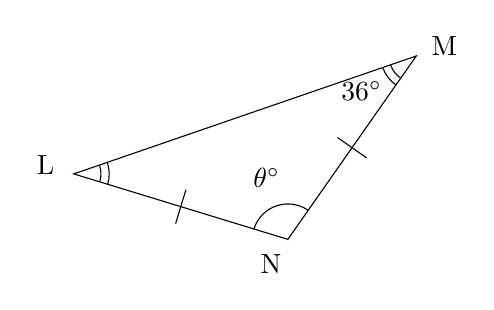
\begin{tikzpicture}[scale=1.5, baseline=(current bounding box.north)]

    \begin{scope}[rotate=199]
      \coordinate (A) at (0,0);
      \coordinate (B) at (3.0664161685590976,0);
      \coordinate (C) at (intersection cs: first line={(A)--($(A)+(36:4cm)$)}, second line={(B)--($(B)+(180-36:4cm)$)});
      \draw (A) -- (B) -- (C) -- cycle;

      % Mark angles with arcs; double arc for equal angles
      \draw ($(A)!0.23cm!(B)$) arc [start angle=0, end angle=36, radius=0.23cm];
      \draw ($(A)!0.3cm!(B)$) arc [start angle=0, end angle=36, radius=0.3cm];
      \draw ($(B)!0.23cm!(C)$) arc [start angle=180-36, end angle=180, radius=0.23cm];
      \draw ($(B)!0.3cm!(C)$) arc [start angle=180-36, end angle=180, radius=0.3cm];
      \draw ($(C)!0.3cm!(A)$) arc [start angle=180+36, end angle=360-36, radius=0.3cm];

      % Label angles
      \node at ($(A)!-0.25cm!(B)$) {M};
      \node at ($(B)!-0.25cm!(C)$) {L};
      \node at ($(C)!-0.25cm!(A)$) {N};

      % Mark angles in degrees
      \coordinate (midBC) at ($(B)!0.5!(C)$);
      \node at ($(A)!0.55cm!(midBC)$) {$36^\circ$};

      \coordinate (midAC) at ($(A)!0.5!(C)$);
      \node at ($(B)!0.55cm!(midAC)$) {};

      \coordinate (midAB) at ($(A)!0.5!(B)$);
      \node at ($(C)!0.55cm!(midAB)$) {$\theta^\circ$};

      % Draw hash mark perpendicular to line AB at its midpoint
      \draw[black] ($(midAC)!1.5mm!90:(A)$)--($(midAC)!1.5mm!-90:(A)$);

      % Add hash marks on side AC
      \draw[black] ($(midBC)!1.5mm!90:(B)$)--($(midBC)!1.5mm!-90:(B)$);

    \end{scope}
  \end{tikzpicture}
\end{minipage}%
\hfill
\begin{minipage}{0.4\textwidth}
  \begin{align*}
    \text{$\theta^\circ$} &= 180^\circ - (\angle \text{M} + \angle \text{L}) \\
    &= 180^\circ - (36^\circ + 36^\circ) \\
    &= 180^\circ - 72^\circ \\
    &= 108^\circ
  \end{align*}
\end{minipage}

\begin{minipage}{0.55\textwidth}
  \refstepcounter{minipagecount}
  \noindent{(\theminipagecount)}\quad
  \begin{tikzpicture}[scale=1.5, baseline=(current bounding box.north)]

    \begin{scope}[rotate=301]
      \coordinate (A) at (0,0);
      \coordinate (B) at (3.550467202902078,0);
      \coordinate (C) at (intersection cs: first line={(A)--($(A)+(62:4cm)$)}, second line={(B)--($(B)+(180-62:4cm)$)});
      \draw (A) -- (B) -- (C) -- cycle;

      % Mark angles with arcs; double arc for equal angles
      \draw ($(A)!0.23cm!(B)$) arc [start angle=0, end angle=62, radius=0.23cm];
      \draw ($(A)!0.3cm!(B)$) arc [start angle=0, end angle=62, radius=0.3cm];
      \draw ($(B)!0.23cm!(C)$) arc [start angle=180-62, end angle=180, radius=0.23cm];
      \draw ($(B)!0.3cm!(C)$) arc [start angle=180-62, end angle=180, radius=0.3cm];
      \draw ($(C)!0.3cm!(A)$) arc [start angle=180+62, end angle=360-62, radius=0.3cm];

      % Label angles
      \node at ($(A)!-0.25cm!(B)$) {X};
      \node at ($(B)!-0.25cm!(C)$) {Z};
      \node at ($(C)!-0.25cm!(A)$) {Y};

      % Mark angles in degrees
      \coordinate (midBC) at ($(B)!0.5!(C)$);
      \node at ($(A)!0.55cm!(midBC)$) {};

      \coordinate (midAC) at ($(A)!0.5!(C)$);
      \node at ($(B)!0.55cm!(midAC)$) {$\theta^\circ$};

      \coordinate (midAB) at ($(A)!0.5!(B)$);
      \node at ($(C)!0.55cm!(midAB)$) {$56^\circ$};

      % Draw hash mark perpendicular to line AB at its midpoint
      \draw[black] ($(midAC)!1.5mm!90:(A)$)--($(midAC)!1.5mm!-90:(A)$);

      % Add hash marks on side AC
      \draw[black] ($(midBC)!1.5mm!90:(B)$)--($(midBC)!1.5mm!-90:(B)$);

    \end{scope}
  \end{tikzpicture}
\end{minipage}%
\hfill
\begin{minipage}{0.4\textwidth}
  \begin{align*}
    \text{$\theta^\circ$} &= \frac{(180^\circ - \angle \text{Y})}{2} \\
    &= \frac{(180^\circ - 56^\circ)}{2} \\
    &= \frac{124^\circ}{2} \\
    &= 62^\circ
  \end{align*}
\end{minipage}

\begin{minipage}{0.55\textwidth}
  \refstepcounter{minipagecount}
  \noindent{(\theminipagecount)}\quad
  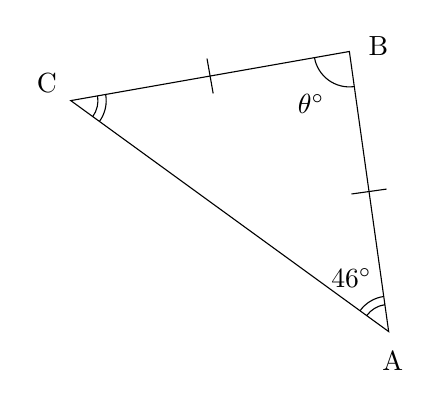
\begin{tikzpicture}[scale=1.5, baseline=(current bounding box.north)]

    \begin{scope}[rotate=324]
      \coordinate (A) at (0,0);
      \coordinate (B) at (3.326476120781351,0);
      \coordinate (C) at (intersection cs: first line={(A)--($(A)+(46:4cm)$)}, second line={(B)--($(B)+(180-46:4cm)$)});
      \draw (A) -- (B) -- (C) -- cycle;

      % Mark angles with arcs; double arc for equal angles
      \draw ($(A)!0.23cm!(B)$) arc [start angle=0, end angle=46, radius=0.23cm];
      \draw ($(A)!0.3cm!(B)$) arc [start angle=0, end angle=46, radius=0.3cm];
      \draw ($(B)!0.23cm!(C)$) arc [start angle=180-46, end angle=180, radius=0.23cm];
      \draw ($(B)!0.3cm!(C)$) arc [start angle=180-46, end angle=180, radius=0.3cm];
      \draw ($(C)!0.3cm!(A)$) arc [start angle=180+46, end angle=360-46, radius=0.3cm];

      % Label angles
      \node at ($(A)!-0.25cm!(B)$) {C};
      \node at ($(B)!-0.25cm!(C)$) {A};
      \node at ($(C)!-0.25cm!(A)$) {B};

      % Mark angles in degrees
      \coordinate (midBC) at ($(B)!0.5!(C)$);
      \node at ($(A)!0.55cm!(midBC)$) {};

      \coordinate (midAC) at ($(A)!0.5!(C)$);
      \node at ($(B)!0.55cm!(midAC)$) {$46^\circ$};

      \coordinate (midAB) at ($(A)!0.5!(B)$);
      \node at ($(C)!0.55cm!(midAB)$) {$\theta^\circ$};

      % Draw hash mark perpendicular to line AB at its midpoint
      \draw[black] ($(midAC)!1.5mm!90:(A)$)--($(midAC)!1.5mm!-90:(A)$);

      % Add hash marks on side AC
      \draw[black] ($(midBC)!1.5mm!90:(B)$)--($(midBC)!1.5mm!-90:(B)$);

    \end{scope}
  \end{tikzpicture}
\end{minipage}%
\hfill
\begin{minipage}{0.4\textwidth}
  \begin{align*}
    \text{$\theta^\circ$} &= 180^\circ - (\angle \text{C} + \angle \text{A}) \\
    &= 180^\circ - (46^\circ + 46^\circ) \\
    &= 180^\circ - 92^\circ \\
    &= 88^\circ
  \end{align*}
\end{minipage}

\begin{minipage}{0.55\textwidth}
  \refstepcounter{minipagecount}
  \noindent{(\theminipagecount)}\quad
  \begin{tikzpicture}[scale=1.5, baseline=(current bounding box.north)]

    \begin{scope}[rotate=255]
      \coordinate (A) at (0,0);
      \coordinate (B) at (3.2381276565662915,0);
      \coordinate (C) at (intersection cs: first line={(A)--($(A)+(43:4cm)$)}, second line={(B)--($(B)+(180-43:4cm)$)});
      \draw (A) -- (B) -- (C) -- cycle;

      % Mark angles with arcs; double arc for equal angles
      \draw ($(A)!0.23cm!(B)$) arc [start angle=0, end angle=43, radius=0.23cm];
      \draw ($(A)!0.3cm!(B)$) arc [start angle=0, end angle=43, radius=0.3cm];
      \draw ($(B)!0.23cm!(C)$) arc [start angle=180-43, end angle=180, radius=0.23cm];
      \draw ($(B)!0.3cm!(C)$) arc [start angle=180-43, end angle=180, radius=0.3cm];
      \draw ($(C)!0.3cm!(A)$) arc [start angle=180+43, end angle=360-43, radius=0.3cm];

      % Label angles
      \node at ($(A)!-0.25cm!(B)$) {C};
      \node at ($(B)!-0.25cm!(C)$) {B};
      \node at ($(C)!-0.25cm!(A)$) {A};

      % Mark angles in degrees
      \coordinate (midBC) at ($(B)!0.5!(C)$);
      \node at ($(A)!0.55cm!(midBC)$) {$43^\circ$};

      \coordinate (midAC) at ($(A)!0.5!(C)$);
      \node at ($(B)!0.55cm!(midAC)$) {};

      \coordinate (midAB) at ($(A)!0.5!(B)$);
      \node at ($(C)!0.55cm!(midAB)$) {$\theta^\circ$};

      % Draw hash mark perpendicular to line AB at its midpoint
      \draw[black] ($(midAC)!1.5mm!90:(A)$)--($(midAC)!1.5mm!-90:(A)$);

      % Add hash marks on side AC
      \draw[black] ($(midBC)!1.5mm!90:(B)$)--($(midBC)!1.5mm!-90:(B)$);

    \end{scope}
  \end{tikzpicture}
\end{minipage}%
\hfill
\begin{minipage}{0.4\textwidth}
  \begin{align*}
    \text{$\theta^\circ$} &= 180^\circ - (\angle \text{C} + \angle \text{B}) \\
    &= 180^\circ - (43^\circ + 43^\circ) \\
    &= 180^\circ - 86^\circ \\
    &= 94^\circ
  \end{align*}
\end{minipage}

\begin{minipage}{0.55\textwidth}
  \refstepcounter{minipagecount}
  \noindent{(\theminipagecount)}\quad
  \begin{tikzpicture}[scale=1.5, baseline=(current bounding box.north)]

    \begin{scope}[rotate=241]
      \coordinate (A) at (0,0);
      \coordinate (B) at (3.4649480770730365,0);
      \coordinate (C) at (intersection cs: first line={(A)--($(A)+(64:4cm)$)}, second line={(B)--($(B)+(180-64:4cm)$)});
      \draw (A) -- (B) -- (C) -- cycle;

      % Mark angles with arcs; double arc for equal angles
      \draw ($(A)!0.23cm!(B)$) arc [start angle=0, end angle=64, radius=0.23cm];
      \draw ($(A)!0.3cm!(B)$) arc [start angle=0, end angle=64, radius=0.3cm];
      \draw ($(B)!0.23cm!(C)$) arc [start angle=180-64, end angle=180, radius=0.23cm];
      \draw ($(B)!0.3cm!(C)$) arc [start angle=180-64, end angle=180, radius=0.3cm];
      \draw ($(C)!0.3cm!(A)$) arc [start angle=180+64, end angle=360-64, radius=0.3cm];

      % Label angles
      \node at ($(A)!-0.25cm!(B)$) {C};
      \node at ($(B)!-0.25cm!(C)$) {B};
      \node at ($(C)!-0.25cm!(A)$) {A};

      % Mark angles in degrees
      \coordinate (midBC) at ($(B)!0.5!(C)$);
      \node at ($(A)!0.55cm!(midBC)$) {$64^\circ$};

      \coordinate (midAC) at ($(A)!0.5!(C)$);
      \node at ($(B)!0.55cm!(midAC)$) {};

      \coordinate (midAB) at ($(A)!0.5!(B)$);
      \node at ($(C)!0.55cm!(midAB)$) {$\theta^\circ$};

      % Draw hash mark perpendicular to line AB at its midpoint
      \draw[black] ($(midAC)!1.5mm!90:(A)$)--($(midAC)!1.5mm!-90:(A)$);

      % Add hash marks on side AC
      \draw[black] ($(midBC)!1.5mm!90:(B)$)--($(midBC)!1.5mm!-90:(B)$);

    \end{scope}
  \end{tikzpicture}
\end{minipage}%
\hfill
\begin{minipage}{0.4\textwidth}
  \begin{align*}
    \text{$\theta^\circ$} &= 180^\circ - (\angle \text{C} + \angle \text{B}) \\
    &= 180^\circ - (64^\circ + 64^\circ) \\
    &= 180^\circ - 128^\circ \\
    &= 52^\circ
  \end{align*}
\end{minipage}

\begin{minipage}{0.55\textwidth}
  \refstepcounter{minipagecount}
  \noindent{(\theminipagecount)}\quad
  \begin{tikzpicture}[scale=1.5, baseline=(current bounding box.north)]

    \begin{scope}[rotate=3]
      \coordinate (A) at (0,0);
      \coordinate (B) at (3.6248019295345557,0);
      \coordinate (C) at (intersection cs: first line={(A)--($(A)+(55:4cm)$)}, second line={(B)--($(B)+(180-55:4cm)$)});
      \draw (A) -- (B) -- (C) -- cycle;

      % Mark angles with arcs; double arc for equal angles
      \draw ($(A)!0.23cm!(B)$) arc [start angle=0, end angle=55, radius=0.23cm];
      \draw ($(A)!0.3cm!(B)$) arc [start angle=0, end angle=55, radius=0.3cm];
      \draw ($(B)!0.23cm!(C)$) arc [start angle=180-55, end angle=180, radius=0.23cm];
      \draw ($(B)!0.3cm!(C)$) arc [start angle=180-55, end angle=180, radius=0.3cm];
      \draw ($(C)!0.3cm!(A)$) arc [start angle=180+55, end angle=360-55, radius=0.3cm];

      % Label angles
      \node at ($(A)!-0.25cm!(B)$) {S};
      \node at ($(B)!-0.25cm!(C)$) {T};
      \node at ($(C)!-0.25cm!(A)$) {R};

      % Mark angles in degrees
      \coordinate (midBC) at ($(B)!0.5!(C)$);
      \node at ($(A)!0.55cm!(midBC)$) {};

      \coordinate (midAC) at ($(A)!0.5!(C)$);
      \node at ($(B)!0.55cm!(midAC)$) {$55^\circ$};

      \coordinate (midAB) at ($(A)!0.5!(B)$);
      \node at ($(C)!0.55cm!(midAB)$) {$\theta^\circ$};

      % Draw hash mark perpendicular to line AB at its midpoint
      \draw[black] ($(midAC)!1.5mm!90:(A)$)--($(midAC)!1.5mm!-90:(A)$);

      % Add hash marks on side AC
      \draw[black] ($(midBC)!1.5mm!90:(B)$)--($(midBC)!1.5mm!-90:(B)$);

    \end{scope}
  \end{tikzpicture}
\end{minipage}%
\hfill
\begin{minipage}{0.4\textwidth}
  \begin{align*}
    \text{$\theta^\circ$} &= 180^\circ - (\angle \text{S} + \angle \text{T}) \\
    &= 180^\circ - (55^\circ + 55^\circ) \\
    &= 180^\circ - 110^\circ \\
    &= 70^\circ
  \end{align*}
\end{minipage}

\begin{minipage}{0.55\textwidth}
  \refstepcounter{minipagecount}
  \noindent{(\theminipagecount)}\quad
  \begin{tikzpicture}[scale=1.5, baseline=(current bounding box.north)]

    \begin{scope}[rotate=58]
      \coordinate (A) at (0,0);
      \coordinate (B) at (3.4533808108364052,0);
      \coordinate (C) at (intersection cs: first line={(A)--($(A)+(48:4cm)$)}, second line={(B)--($(B)+(180-48:4cm)$)});
      \draw (A) -- (B) -- (C) -- cycle;

      % Mark angles with arcs; double arc for equal angles
      \draw ($(A)!0.23cm!(B)$) arc [start angle=0, end angle=48, radius=0.23cm];
      \draw ($(A)!0.3cm!(B)$) arc [start angle=0, end angle=48, radius=0.3cm];
      \draw ($(B)!0.23cm!(C)$) arc [start angle=180-48, end angle=180, radius=0.23cm];
      \draw ($(B)!0.3cm!(C)$) arc [start angle=180-48, end angle=180, radius=0.3cm];
      \draw ($(C)!0.3cm!(A)$) arc [start angle=180+48, end angle=360-48, radius=0.3cm];

      % Label angles
      \node at ($(A)!-0.25cm!(B)$) {R};
      \node at ($(B)!-0.25cm!(C)$) {T};
      \node at ($(C)!-0.25cm!(A)$) {S};

      % Mark angles in degrees
      \coordinate (midBC) at ($(B)!0.5!(C)$);
      \node at ($(A)!0.55cm!(midBC)$) {$48^\circ$};

      \coordinate (midAC) at ($(A)!0.5!(C)$);
      \node at ($(B)!0.55cm!(midAC)$) {};

      \coordinate (midAB) at ($(A)!0.5!(B)$);
      \node at ($(C)!0.55cm!(midAB)$) {$\theta^\circ$};

      % Draw hash mark perpendicular to line AB at its midpoint
      \draw[black] ($(midAC)!1.5mm!90:(A)$)--($(midAC)!1.5mm!-90:(A)$);

      % Add hash marks on side AC
      \draw[black] ($(midBC)!1.5mm!90:(B)$)--($(midBC)!1.5mm!-90:(B)$);

    \end{scope}
  \end{tikzpicture}
\end{minipage}%
\hfill
\begin{minipage}{0.4\textwidth}
  \begin{align*}
    \text{$\theta^\circ$} &= 180^\circ - (\angle \text{R} + \angle \text{T}) \\
    &= 180^\circ - (48^\circ + 48^\circ) \\
    &= 180^\circ - 96^\circ \\
    &= 84^\circ
  \end{align*}
\end{minipage}

\begin{minipage}{0.55\textwidth}
  \refstepcounter{minipagecount}
  \noindent{(\theminipagecount)}\quad
  \begin{tikzpicture}[scale=1.5, baseline=(current bounding box.north)]

    \begin{scope}[rotate=25]
      \coordinate (A) at (0,0);
      \coordinate (B) at (3.606909340979945,0);
      \coordinate (C) at (intersection cs: first line={(A)--($(A)+(61:4cm)$)}, second line={(B)--($(B)+(180-61:4cm)$)});
      \draw (A) -- (B) -- (C) -- cycle;

      % Mark angles with arcs; double arc for equal angles
      \draw ($(A)!0.23cm!(B)$) arc [start angle=0, end angle=61, radius=0.23cm];
      \draw ($(A)!0.3cm!(B)$) arc [start angle=0, end angle=61, radius=0.3cm];
      \draw ($(B)!0.23cm!(C)$) arc [start angle=180-61, end angle=180, radius=0.23cm];
      \draw ($(B)!0.3cm!(C)$) arc [start angle=180-61, end angle=180, radius=0.3cm];
      \draw ($(C)!0.3cm!(A)$) arc [start angle=180+61, end angle=360-61, radius=0.3cm];

      % Label angles
      \node at ($(A)!-0.25cm!(B)$) {B};
      \node at ($(B)!-0.25cm!(C)$) {A};
      \node at ($(C)!-0.25cm!(A)$) {C};

      % Mark angles in degrees
      \coordinate (midBC) at ($(B)!0.5!(C)$);
      \node at ($(A)!0.55cm!(midBC)$) {};

      \coordinate (midAC) at ($(A)!0.5!(C)$);
      \node at ($(B)!0.55cm!(midAC)$) {$\theta^\circ$};

      \coordinate (midAB) at ($(A)!0.5!(B)$);
      \node at ($(C)!0.55cm!(midAB)$) {$58^\circ$};

      % Draw hash mark perpendicular to line AB at its midpoint
      \draw[black] ($(midAC)!1.5mm!90:(A)$)--($(midAC)!1.5mm!-90:(A)$);

      % Add hash marks on side AC
      \draw[black] ($(midBC)!1.5mm!90:(B)$)--($(midBC)!1.5mm!-90:(B)$);

    \end{scope}
  \end{tikzpicture}
\end{minipage}%
\hfill
\begin{minipage}{0.4\textwidth}
  \begin{align*}
    \text{$\theta^\circ$} &= \frac{(180^\circ - \angle \text{C})}{2} \\
    &= \frac{(180^\circ - 58^\circ)}{2} \\
    &= \frac{122^\circ}{2} \\
    &= 61^\circ
  \end{align*}
\end{minipage}

\begin{minipage}{0.55\textwidth}
  \refstepcounter{minipagecount}
  \noindent{(\theminipagecount)}\quad
  \begin{tikzpicture}[scale=1.5, baseline=(current bounding box.north)]

    \begin{scope}[rotate=312]
      \coordinate (A) at (0,0);
      \coordinate (B) at (3.2778891459611605,0);
      \coordinate (C) at (intersection cs: first line={(A)--($(A)+(44:4cm)$)}, second line={(B)--($(B)+(180-44:4cm)$)});
      \draw (A) -- (B) -- (C) -- cycle;

      % Mark angles with arcs; double arc for equal angles
      \draw ($(A)!0.23cm!(B)$) arc [start angle=0, end angle=44, radius=0.23cm];
      \draw ($(A)!0.3cm!(B)$) arc [start angle=0, end angle=44, radius=0.3cm];
      \draw ($(B)!0.23cm!(C)$) arc [start angle=180-44, end angle=180, radius=0.23cm];
      \draw ($(B)!0.3cm!(C)$) arc [start angle=180-44, end angle=180, radius=0.3cm];
      \draw ($(C)!0.3cm!(A)$) arc [start angle=180+44, end angle=360-44, radius=0.3cm];

      % Label angles
      \node at ($(A)!-0.25cm!(B)$) {C};
      \node at ($(B)!-0.25cm!(C)$) {B};
      \node at ($(C)!-0.25cm!(A)$) {A};

      % Mark angles in degrees
      \coordinate (midBC) at ($(B)!0.5!(C)$);
      \node at ($(A)!0.55cm!(midBC)$) {$\theta^\circ$};

      \coordinate (midAC) at ($(A)!0.5!(C)$);
      \node at ($(B)!0.55cm!(midAC)$) {};

      \coordinate (midAB) at ($(A)!0.5!(B)$);
      \node at ($(C)!0.55cm!(midAB)$) {$92^\circ$};

      % Draw hash mark perpendicular to line AB at its midpoint
      \draw[black] ($(midAC)!1.5mm!90:(A)$)--($(midAC)!1.5mm!-90:(A)$);

      % Add hash marks on side AC
      \draw[black] ($(midBC)!1.5mm!90:(B)$)--($(midBC)!1.5mm!-90:(B)$);

    \end{scope}
  \end{tikzpicture}
\end{minipage}%
\hfill
\begin{minipage}{0.4\textwidth}
  \begin{align*}
    \text{$\theta^\circ$} &= \frac{(180^\circ - \angle \text{A})}{2} \\
    &= \frac{(180^\circ - 92^\circ)}{2} \\
    &= \frac{88^\circ}{2} \\
    &= 44^\circ
  \end{align*}
\end{minipage}

\begin{minipage}{0.55\textwidth}
  \refstepcounter{minipagecount}
  \noindent{(\theminipagecount)}\quad
  \begin{tikzpicture}[scale=1.5, baseline=(current bounding box.north)]

    \begin{scope}[rotate=58]
      \coordinate (A) at (0,0);
      \coordinate (B) at (3.3414709886830494,0);
      \coordinate (C) at (intersection cs: first line={(A)--($(A)+(54:4cm)$)}, second line={(B)--($(B)+(180-54:4cm)$)});
      \draw (A) -- (B) -- (C) -- cycle;

      % Mark angles with arcs; double arc for equal angles
      \draw ($(A)!0.23cm!(B)$) arc [start angle=0, end angle=54, radius=0.23cm];
      \draw ($(A)!0.3cm!(B)$) arc [start angle=0, end angle=54, radius=0.3cm];
      \draw ($(B)!0.23cm!(C)$) arc [start angle=180-54, end angle=180, radius=0.23cm];
      \draw ($(B)!0.3cm!(C)$) arc [start angle=180-54, end angle=180, radius=0.3cm];
      \draw ($(C)!0.3cm!(A)$) arc [start angle=180+54, end angle=360-54, radius=0.3cm];

      % Label angles
      \node at ($(A)!-0.25cm!(B)$) {L};
      \node at ($(B)!-0.25cm!(C)$) {M};
      \node at ($(C)!-0.25cm!(A)$) {N};

      % Mark angles in degrees
      \coordinate (midBC) at ($(B)!0.5!(C)$);
      \node at ($(A)!0.55cm!(midBC)$) {$\theta^\circ$};

      \coordinate (midAC) at ($(A)!0.5!(C)$);
      \node at ($(B)!0.55cm!(midAC)$) {};

      \coordinate (midAB) at ($(A)!0.5!(B)$);
      \node at ($(C)!0.55cm!(midAB)$) {$72^\circ$};

      % Draw hash mark perpendicular to line AB at its midpoint
      \draw[black] ($(midAC)!1.5mm!90:(A)$)--($(midAC)!1.5mm!-90:(A)$);

      % Add hash marks on side AC
      \draw[black] ($(midBC)!1.5mm!90:(B)$)--($(midBC)!1.5mm!-90:(B)$);

    \end{scope}
  \end{tikzpicture}
\end{minipage}%
\hfill
\begin{minipage}{0.4\textwidth}
  \begin{align*}
    \text{$\theta^\circ$} &= \frac{(180^\circ - \angle \text{N})}{2} \\
    &= \frac{(180^\circ - 72^\circ)}{2} \\
    &= \frac{108^\circ}{2} \\
    &= 54^\circ
  \end{align*}
\end{minipage}

\begin{minipage}{0.55\textwidth}
  \refstepcounter{minipagecount}
  \noindent{(\theminipagecount)}\quad
  \begin{tikzpicture}[scale=1.5, baseline=(current bounding box.north)]

    \begin{scope}[rotate=268]
      \coordinate (A) at (0,0);
      \coordinate (B) at (3.989110756926936,0);
      \coordinate (C) at (intersection cs: first line={(A)--($(A)+(59:4cm)$)}, second line={(B)--($(B)+(180-59:4cm)$)});
      \draw (A) -- (B) -- (C) -- cycle;

      % Mark angles with arcs; double arc for equal angles
      \draw ($(A)!0.23cm!(B)$) arc [start angle=0, end angle=59, radius=0.23cm];
      \draw ($(A)!0.3cm!(B)$) arc [start angle=0, end angle=59, radius=0.3cm];
      \draw ($(B)!0.23cm!(C)$) arc [start angle=180-59, end angle=180, radius=0.23cm];
      \draw ($(B)!0.3cm!(C)$) arc [start angle=180-59, end angle=180, radius=0.3cm];
      \draw ($(C)!0.3cm!(A)$) arc [start angle=180+59, end angle=360-59, radius=0.3cm];

      % Label angles
      \node at ($(A)!-0.25cm!(B)$) {N};
      \node at ($(B)!-0.25cm!(C)$) {M};
      \node at ($(C)!-0.25cm!(A)$) {L};

      % Mark angles in degrees
      \coordinate (midBC) at ($(B)!0.5!(C)$);
      \node at ($(A)!0.55cm!(midBC)$) {$59^\circ$};

      \coordinate (midAC) at ($(A)!0.5!(C)$);
      \node at ($(B)!0.55cm!(midAC)$) {};

      \coordinate (midAB) at ($(A)!0.5!(B)$);
      \node at ($(C)!0.55cm!(midAB)$) {$\theta^\circ$};

      % Draw hash mark perpendicular to line AB at its midpoint
      \draw[black] ($(midAC)!1.5mm!90:(A)$)--($(midAC)!1.5mm!-90:(A)$);

      % Add hash marks on side AC
      \draw[black] ($(midBC)!1.5mm!90:(B)$)--($(midBC)!1.5mm!-90:(B)$);

    \end{scope}
  \end{tikzpicture}
\end{minipage}%
\hfill
\begin{minipage}{0.4\textwidth}
  \begin{align*}
    \text{$\theta^\circ$} &= 180^\circ - (\angle \text{N} + \angle \text{M}) \\
    &= 180^\circ - (59^\circ + 59^\circ) \\
    &= 180^\circ - 118^\circ \\
    &= 62^\circ
  \end{align*}
\end{minipage}

\begin{minipage}{0.55\textwidth}
  \refstepcounter{minipagecount}
  \noindent{(\theminipagecount)}\quad
  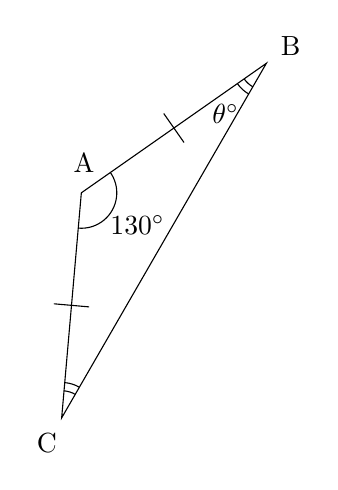
\begin{tikzpicture}[scale=1.5, baseline=(current bounding box.north)]

    \begin{scope}[rotate=60]
      \coordinate (A) at (0,0);
      \coordinate (B) at (3.4664015205586622,0);
      \coordinate (C) at (intersection cs: first line={(A)--($(A)+(25:4cm)$)}, second line={(B)--($(B)+(180-25:4cm)$)});
      \draw (A) -- (B) -- (C) -- cycle;

      % Mark angles with arcs; double arc for equal angles
      \draw ($(A)!0.23cm!(B)$) arc [start angle=0, end angle=25, radius=0.23cm];
      \draw ($(A)!0.3cm!(B)$) arc [start angle=0, end angle=25, radius=0.3cm];
      \draw ($(B)!0.23cm!(C)$) arc [start angle=180-25, end angle=180, radius=0.23cm];
      \draw ($(B)!0.3cm!(C)$) arc [start angle=180-25, end angle=180, radius=0.3cm];
      \draw ($(C)!0.3cm!(A)$) arc [start angle=180+25, end angle=360-25, radius=0.3cm];

      % Label angles
      \node at ($(A)!-0.25cm!(B)$) {C};
      \node at ($(B)!-0.25cm!(C)$) {B};
      \node at ($(C)!-0.25cm!(A)$) {A};

      % Mark angles in degrees
      \coordinate (midBC) at ($(B)!0.5!(C)$);
      \node at ($(A)!0.55cm!(midBC)$) {};

      \coordinate (midAC) at ($(A)!0.5!(C)$);
      \node at ($(B)!0.55cm!(midAC)$) {$\theta^\circ$};

      \coordinate (midAB) at ($(A)!0.5!(B)$);
      \node at ($(C)!0.55cm!(midAB)$) {$130^\circ$};

      % Draw hash mark perpendicular to line AB at its midpoint
      \draw[black] ($(midAC)!1.5mm!90:(A)$)--($(midAC)!1.5mm!-90:(A)$);

      % Add hash marks on side AC
      \draw[black] ($(midBC)!1.5mm!90:(B)$)--($(midBC)!1.5mm!-90:(B)$);

    \end{scope}
  \end{tikzpicture}
\end{minipage}%
\hfill
\begin{minipage}{0.4\textwidth}
  \begin{align*}
    \text{$\theta^\circ$} &= \frac{(180^\circ - \angle \text{A})}{2} \\
    &= \frac{(180^\circ - 130^\circ)}{2} \\
    &= \frac{50^\circ}{2} \\
    &= 25^\circ
  \end{align*}
\end{minipage}

\begin{minipage}{0.55\textwidth}
  \refstepcounter{minipagecount}
  \noindent{(\theminipagecount)}\quad
  \begin{tikzpicture}[scale=1.5, baseline=(current bounding box.north)]

    \begin{scope}[rotate=120]
      \coordinate (A) at (0,0);
      \coordinate (B) at (3.995682249069551,0);
      \coordinate (C) at (intersection cs: first line={(A)--($(A)+(37:4cm)$)}, second line={(B)--($(B)+(180-37:4cm)$)});
      \draw (A) -- (B) -- (C) -- cycle;

      % Mark angles with arcs; double arc for equal angles
      \draw ($(A)!0.23cm!(B)$) arc [start angle=0, end angle=37, radius=0.23cm];
      \draw ($(A)!0.3cm!(B)$) arc [start angle=0, end angle=37, radius=0.3cm];
      \draw ($(B)!0.23cm!(C)$) arc [start angle=180-37, end angle=180, radius=0.23cm];
      \draw ($(B)!0.3cm!(C)$) arc [start angle=180-37, end angle=180, radius=0.3cm];
      \draw ($(C)!0.3cm!(A)$) arc [start angle=180+37, end angle=360-37, radius=0.3cm];

      % Label angles
      \node at ($(A)!-0.25cm!(B)$) {Z};
      \node at ($(B)!-0.25cm!(C)$) {X};
      \node at ($(C)!-0.25cm!(A)$) {Y};

      % Mark angles in degrees
      \coordinate (midBC) at ($(B)!0.5!(C)$);
      \node at ($(A)!0.55cm!(midBC)$) {$37^\circ$};

      \coordinate (midAC) at ($(A)!0.5!(C)$);
      \node at ($(B)!0.55cm!(midAC)$) {};

      \coordinate (midAB) at ($(A)!0.5!(B)$);
      \node at ($(C)!0.55cm!(midAB)$) {$\theta^\circ$};

      % Draw hash mark perpendicular to line AB at its midpoint
      \draw[black] ($(midAC)!1.5mm!90:(A)$)--($(midAC)!1.5mm!-90:(A)$);

      % Add hash marks on side AC
      \draw[black] ($(midBC)!1.5mm!90:(B)$)--($(midBC)!1.5mm!-90:(B)$);

    \end{scope}
  \end{tikzpicture}
\end{minipage}%
\hfill
\begin{minipage}{0.4\textwidth}
  \begin{align*}
    \text{$\theta^\circ$} &= 180^\circ - (\angle \text{Z} + \angle \text{X}) \\
    &= 180^\circ - (37^\circ + 37^\circ) \\
    &= 180^\circ - 74^\circ \\
    &= 106^\circ
  \end{align*}
\end{minipage}

\begin{minipage}{0.55\textwidth}
  \refstepcounter{minipagecount}
  \noindent{(\theminipagecount)}\quad
  \begin{tikzpicture}[scale=1.5, baseline=(current bounding box.north)]

    \begin{scope}[rotate=294]
      \coordinate (A) at (0,0);
      \coordinate (B) at (3.1958293459108207,0);
      \coordinate (C) at (intersection cs: first line={(A)--($(A)+(41:4cm)$)}, second line={(B)--($(B)+(180-41:4cm)$)});
      \draw (A) -- (B) -- (C) -- cycle;

      % Mark angles with arcs; double arc for equal angles
      \draw ($(A)!0.23cm!(B)$) arc [start angle=0, end angle=41, radius=0.23cm];
      \draw ($(A)!0.3cm!(B)$) arc [start angle=0, end angle=41, radius=0.3cm];
      \draw ($(B)!0.23cm!(C)$) arc [start angle=180-41, end angle=180, radius=0.23cm];
      \draw ($(B)!0.3cm!(C)$) arc [start angle=180-41, end angle=180, radius=0.3cm];
      \draw ($(C)!0.3cm!(A)$) arc [start angle=180+41, end angle=360-41, radius=0.3cm];

      % Label angles
      \node at ($(A)!-0.25cm!(B)$) {R};
      \node at ($(B)!-0.25cm!(C)$) {S};
      \node at ($(C)!-0.25cm!(A)$) {T};

      % Mark angles in degrees
      \coordinate (midBC) at ($(B)!0.5!(C)$);
      \node at ($(A)!0.55cm!(midBC)$) {};

      \coordinate (midAC) at ($(A)!0.5!(C)$);
      \node at ($(B)!0.55cm!(midAC)$) {$\theta^\circ$};

      \coordinate (midAB) at ($(A)!0.5!(B)$);
      \node at ($(C)!0.55cm!(midAB)$) {$98^\circ$};

      % Draw hash mark perpendicular to line AB at its midpoint
      \draw[black] ($(midAC)!1.5mm!90:(A)$)--($(midAC)!1.5mm!-90:(A)$);

      % Add hash marks on side AC
      \draw[black] ($(midBC)!1.5mm!90:(B)$)--($(midBC)!1.5mm!-90:(B)$);

    \end{scope}
  \end{tikzpicture}
\end{minipage}%
\hfill
\begin{minipage}{0.4\textwidth}
  \begin{align*}
    \text{$\theta^\circ$} &= \frac{(180^\circ - \angle \text{T})}{2} \\
    &= \frac{(180^\circ - 98^\circ)}{2} \\
    &= \frac{82^\circ}{2} \\
    &= 41^\circ
  \end{align*}
\end{minipage}

\begin{minipage}{0.55\textwidth}
  \refstepcounter{minipagecount}
  \noindent{(\theminipagecount)}\quad
  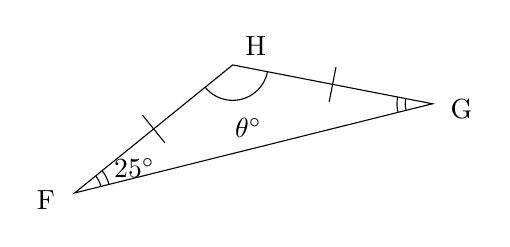
\begin{tikzpicture}[scale=1.5, baseline=(current bounding box.north)]

    \begin{scope}[rotate=14]
      \coordinate (A) at (0,0);
      \coordinate (B) at (3.1219129629741484,0);
      \coordinate (C) at (intersection cs: first line={(A)--($(A)+(25:4cm)$)}, second line={(B)--($(B)+(180-25:4cm)$)});
      \draw (A) -- (B) -- (C) -- cycle;

      % Mark angles with arcs; double arc for equal angles
      \draw ($(A)!0.23cm!(B)$) arc [start angle=0, end angle=25, radius=0.23cm];
      \draw ($(A)!0.3cm!(B)$) arc [start angle=0, end angle=25, radius=0.3cm];
      \draw ($(B)!0.23cm!(C)$) arc [start angle=180-25, end angle=180, radius=0.23cm];
      \draw ($(B)!0.3cm!(C)$) arc [start angle=180-25, end angle=180, radius=0.3cm];
      \draw ($(C)!0.3cm!(A)$) arc [start angle=180+25, end angle=360-25, radius=0.3cm];

      % Label angles
      \node at ($(A)!-0.25cm!(B)$) {F};
      \node at ($(B)!-0.25cm!(C)$) {G};
      \node at ($(C)!-0.25cm!(A)$) {H};

      % Mark angles in degrees
      \coordinate (midBC) at ($(B)!0.5!(C)$);
      \node at ($(A)!0.55cm!(midBC)$) {$25^\circ$};

      \coordinate (midAC) at ($(A)!0.5!(C)$);
      \node at ($(B)!0.55cm!(midAC)$) {};

      \coordinate (midAB) at ($(A)!0.5!(B)$);
      \node at ($(C)!0.55cm!(midAB)$) {$\theta^\circ$};

      % Draw hash mark perpendicular to line AB at its midpoint
      \draw[black] ($(midAC)!1.5mm!90:(A)$)--($(midAC)!1.5mm!-90:(A)$);

      % Add hash marks on side AC
      \draw[black] ($(midBC)!1.5mm!90:(B)$)--($(midBC)!1.5mm!-90:(B)$);

    \end{scope}
  \end{tikzpicture}
\end{minipage}%
\hfill
\begin{minipage}{0.4\textwidth}
  \begin{align*}
    \text{$\theta^\circ$} &= 180^\circ - (\angle \text{F} + \angle \text{G}) \\
    &= 180^\circ - (25^\circ + 25^\circ) \\
    &= 180^\circ - 50^\circ \\
    &= 130^\circ
  \end{align*}
\end{minipage}



\end{document}
